\documentclass[a4paper,12pt]{article}
\usepackage[utf8]{inputenc}

\usepackage[utf8]{inputenc}
\usepackage[T2A]{fontenc}
\usepackage[english,russian]{babel}
\usepackage{amsthm}
\usepackage{amsmath}
\usepackage{amssymb}
\usepackage{tikz}
\usepackage{textcomp}
\usepackage{marvosym}
\usepackage{ esint }
\usepackage{mathtext}
\usepackage{siunitx} % Required for alignment
\usepackage{subfigure}
\usepackage{multirow}
\usepackage{rotating}
\usepackage{afterpage}
\usepackage[arrowdel]{physics}
\usepackage{booktabs}
\setlength{\topmargin}{-0.5in}
\setlength{\textheight}{9.1in}
\setlength{\oddsidemargin}{-0.4in}
\setlength{\evensidemargin}{-0.4in}
\setlength{\textwidth}{7in}
\setlength{\parindent}{0ex}
\setlength{\parskip}{1ex}
\newcommand{\ndiv}{\hspace{-4pt}\not|\hspace{2pt}}
\usepackage{graphicx}
\usepackage{float}
\usepackage{wrapfig}
\usepackage{pgfplots}
\usepackage{caption}
\pgfplotsset{compat=1.16}
\graphicspath{ {./images/} }
\usepackage{graphicx}
\RequirePackage{caption}
\DeclareCaptionLabelSeparator{defffis}{ — }
\captionsetup{justification=centering,labelsep=defffis}
\usepackage{caption} \captionsetup[table]{labelsep=endash,justification=justified,singlelinecheck=false,font=normalsize}
\usepackage{amsfonts,mathtools}

\title{Лабораторная работа № 3.7.1\\Скин-эффект в полом цилиндре}
\author{Илья Прамский}
\date{Ноябрь 2023}

\begin{document}

\maketitle
\newpage
\section*{Введение}
\textbf{Цель работы:} Исследование проникновения переменного магнитного поля в медный полый цилиндр

\section{Теоретическая часть}
\subsection{Скин-эффект для полупрастранства}
\vspace{1cm}
\begin{wrapfigure}{l}{0.3\textwidth}
  \begin{center}
    \includegraphics[width=0.28\textwidth]{poluprostranstvo}
  \end{center}
  \caption{Скин-эффект в полупространстве}\label{fig:poluprostranstvo}
\end{wrapfigure}

Рассмотрим квазистационарное поле внутри проводящей среды в простейшем плоском случае.
Пусть вектор $\vb*{E}$ направлен всюду вдоль оси $y$ (рис. 1) 
и зависит только от координаты $x$, т. е. ${E_x} = {E_z} \equiv 0$, $E_y=E_y(x,t)$.
В квазистационарном приближении 
\begin{equation*}
    \grad \times \vb*{H} = \sigma \vb*{E}
\end{equation*}
Берем ротор обоих частей
\begin{equation*}
    \grad \times (\grad \times \vb*{H}) = \grad(\grad \cdot \vb*{H}) - \grad^2\vb*{H} = \sigma \grad \times \vb*{E}
\end{equation*}
Испоьзуя ур-е Максвелла для ротора $\vb*{E}$ и для дивергенчии $\vb*{H}$ получаем
\begin{equation}
    \grad^2 \vb*{H} = \sigma\mu\mu_0\frac{\partial\vb*{H}}{\partial t} 
                      + \grad(\grad \cdot \vb*{H}) = \sigma\mu\mu_0\frac{\partial\vb*{H}}{\partial t} 
    \label{eq:laplacian_H}
\end{equation}
Берем ротор еще раз
\begin{equation*}
    \grad \times (\grad^2\vb*{H}) = \grad^2 (\grad \times \vb*{H}) =
    \sigma\mu\mu_0 \frac{\partial (\grad \times \vb*{H})}{\partial t}
\end{equation*}
Осталось подставить первое ур-е, и воспользоватся уравнением Максвелла
\begin{equation}
    \grad^2\vb*{E}=\sigma\mu\mu_0 \frac{\partial \vb*{E}}{\partial t}\label{eq:diffusion}
\end{equation}

Подставляем в (\ref{eq:diffusion}) наше электрическое поле $E_y=E_y(x,t)$
\begin{equation}
    \frac{\partial^2 E_y}{\partial x^2} = \sigma\mu\mu_0\frac{\partial E_y}{\partial t}
    \label{eq:diffusion_chastni}
\end{equation}
Если $E_y(0,t)=E_0 e^{i\omega t}$ то решением (\ref{eq:diffusion_chastni}) будет функция вида
\begin{equation}
    E_y(x,t)=E_0 e^{-x/\delta} e^{i(\omega t - x/\delta)}
    \label{eq:skin_effect_poluprostranstvo}
\end{equation}
где
\begin{equation}
    \delta = \sqrt{\frac{2}{\omega\sigma\mu\mu_0}}
    \label{eq:delta}
\end{equation}

\newpage
\subsection{Скин-эффект в тонком полом цилиндре}
\vspace{1cm}
\begin{wrapfigure}[36]{l}{0.3\textwidth}
  \begin{center}
    \includegraphics[width=0.28\textwidth]{cilindr}
  \end{center}
  \caption{Эл-магнитные поля в цилиндре}\label{fig:cilindr}

  \begin{center}
    \includegraphics[width=0.28\textwidth]{stenka}
  \end{center}
  \caption{Стенка цилиндра}\label{fig:stenka}
\end{wrapfigure}

Перейдем теперь к описанию теории в нашей работе. Из соображении симметрии и 
непрерывности соответствующих компонет векторов $\vb*{E}$ и $\vb*{H}$ можем сказать что
\begin{equation*}
    H_z = H(r)e^{i\omega t} \text{, } E_\varphi = E(r)e^{i\omega t}
\end{equation*}
и при этом функции $H(r)$ и $E(r)$ непрерывны.

Внутри цилиндра токов нет, следовательно $H(r)=H_1=\text{const}$ внутри цилиндра.
По теореме об электромагнитной индукции
\begin{equation*}
    E(r) = -\frac{1}{2}\mu_0 r \cdot i \omega H_1
\end{equation*}
откуда мы получаем граничное условие
\begin{equation}
    E_1=E(a)= -\frac{1}{2}\mu_0 a \cdot i \omega H_1
    \label{eq:granichnoe_uslovie_E}
\end{equation}

В прближении $h \ll a$ можем пренебречь кривизной стенки и смоделировать 
его бесконечной полосой. Тогда, надо решить уравнение (\ref{eq:laplacian_H})
с граничными условиями. Решая уравнение получим связь полей $H_1$ 
(поле внутри цилиндра которое мы будем измерять) и $H_2$, которое колебается с частотой
$\omega$

\begin{equation}
    H_1 = \frac{H_0}{\ch(\alpha h) + \frac{1}{2} \alpha a \sh(\alpha h)} 
    \text{\ \ \ }
    \alpha = \sqrt{i\omega \sigma \mu_0} = \frac{\sqrt{2}}{\delta}e^{i\pi/4}
    \label{eq:svyaz_poley}
\end{equation}

из этой формулы получим сколько по фазе отстает поле $H_1$ от $H_0$. При $\delta \ll h$
(высокочастотная область)

\begin{equation}
    \psi \approx \frac{\pi}{4} + \frac{h}{\delta} = 
    \frac{\pi}{4} + h \sqrt{\frac{\omega \sigma \mu_0}{2}}
    \label{eq:faza_high_freq}
\end{equation}

При $\delta \gg h$ (низкочастотная область)

\begin{equation}
    \tan \psi \approx \frac{ah}{\delta^2} = \pi a h \sigma \mu \mu_0 \nu
    \label{eq:faza_low_freq}
\end{equation}
\newpage

\subsection{Процесс измерения}
\begin{wrapfigure}{l}{0.5\textwidth}
  \begin{center}
    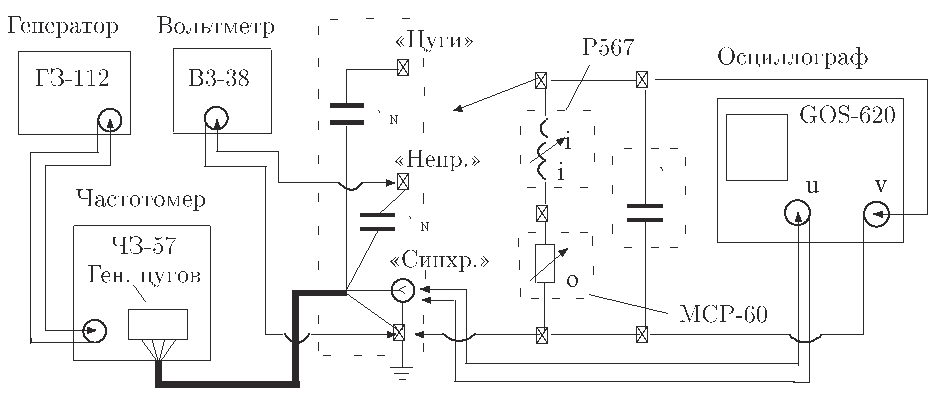
\includegraphics[width=0.48\textwidth]{ustanovka}
  \end{center}
  \caption{Установка}\label{fig:ustanovka}
\end{wrapfigure}

Мангнитное поле внутри цилиндра измеряется катушкой 3. Напряжение на катушке
пропорционалньна производной $\dot{B_1}(t)$
\begin{equation*}
    U(t) \propto \dot{B_1}(t) = -i\omega H_1 e^{i\omega t}
\end{equation*}
Поле внутри цилиндра пропорциональна току через соленоид
\begin{equation*}
    B_0(t) \propto I(t)
\end{equation*}
Отсюда несложно увидеть, что
\begin{equation}
    \frac{\abs{H_1}}{\abs{H_0}} = c \cdot \frac{U}{\nu I} = c \xi
    \label{eq:otnoshenie_amplitud}
\end{equation}
\vspace{0.3cm}

где константу можно определить из условия $\abs{H_1}/\abs{H_2} \rightarrow 1$ при
$\nu \rightarrow 0$.

\vspace{0.3cm}

При измерениях разности фаз нужно учесть, что первый сигнал на осциллографе
пропорционален магнитному полю снаружи, а второй пропорционален производному
поля внутри цилиндра по времени. Вследствии этого набегает дополнительная фаза $\pi/2$,
которую надо вычесть при измерениях.

\section{Ход работы}
Параметры установки 2a = 45мм, h = 1,5мм. Примем проводимость равной порядка $\sigma ~ 5 \cdot 10^7$. Тогда частота, при которой глубина проникновения будет равна толщине стенки h равна $\nu_h = 2252$ Гц.

\subsection{Вычисление проводимости}
Рассмотрим область низких частот($<0,05\nu_h$). Тогда $\nu \ll \nu_h$, а значит $\alpha h \ll 1$, поэтому формулу (\ref{eq:svyaz_poley})  можно представить в виде(учтем, что $\ch{\alpha h} \approx 1, \sh{\alpha h} \approx \alpha h)$

\begin{equation}
	H_1 = \frac{H_0}{1 + \frac{1}{2} \cdot \alpha^2 \cdot a \cdot h}
    \label{eq:svyas_poley_low_freq}
\end{equation}

Тогда отношение модулей $H_1$ и $H_0$ можно представить в виде
\[\frac{|H_1|}{|H_0|} = \frac{1}{\sqrt{1+(\frac{1}{2} \cdot a \cdot h \cdot \omega \cdot \sigma \cdot \mu_0)^2}} = c \xi\]
Что позволяет нам найти зависимость $\frac{1}{\xi^2}$ от $\nu^2$(подставим $\omega = 2 \pi \nu$)
\[\frac{1}{c^2\xi^2} = 1 + (a \cdot h \cdot \sigma \cdot \mu_0)^2 \cdot \nu^2\]
\[\frac{1}{\xi^2} = c^2 + (a \cdot h \cdot \sigma \cdot \mu_0 \cdot c)^2 \cdot \nu^2\]
Теперь построим график зависимости $\frac{1}{\xi^2}$ от $\nu^2$ и убедимся в её линейности.
\begin{figure}[H]
	\begin{center}
    \includegraphics[width=.75\textwidth]{tabliza1.jpg}
	\end{center}
\end{figure}
\begin{figure}[H]
	\begin{center}
    \includegraphics[width=1\textwidth]{graphik1.jpg}
	\end{center}
\end{figure}
Получается, что $c = 72,24 \pm 0,07$ Ом/Гц, а $\sigma = (4,41 \pm 0,02) \cdot 10^7$ См/м.

Далее исследуем зависимость $\xi$ и $\psi$ от частоты $\nu$ при низких частотах(от $0,05 \nu_h$ до $0,5 \nu_h$). Полученные данные занесём в таблицу. По этим результатам построим график зависимости $\tan \psi$ от $\nu$.

Как было сказано выше(из формулы (\ref{eq:faza_low_freq})) следует:
\[\tan\psi \approx ah\pi\sigma\mu_0 \cdot \nu\]
\[\sigma = \frac{k}{ah\pi\mu_0}\]

\begin{figure}[H]
	\begin{center}	\includegraphics[width=0.75\textwidth]{tabliza2.jpg}
	\end{center}
\end{figure}

\begin{figure}[H]
	\begin{center}	\includegraphics[width=1\textwidth]{graphik2.jpg}
	\end{center}
\end{figure}

$k = (6,1 \pm 0,3) \cdot 10^{-3}$ Гц$^{-1}$. $\sigma = (4,7 \pm 0,2) \cdot 10^7$ См/м.

Теперь рассмотрим более высокие частоты. В этой области из формулы (\ref{eq:faza_high_freq}) выполняется следующее равенство
\[\psi - \frac{\pi}{4} = h\sqrt{\pi \sigma \mu_0} \cdot \sqrt{\nu}\]
\[\psi - \frac{\pi}{4} = k_1 \cdot \sqrt{\nu}\]
\[\sigma = \frac{k_1^2}{h^2\pi \mu_0}\]
Повторим измерения на высоких частотах. Внесем полученные данные в таблицу и построим график зависимости $\psi - \frac{\pi}{4}$ от $\sqrt{\nu}$.

\begin{figure}[H]
	\begin{center}	\includegraphics[width=0.75\textwidth]{tabliza3.jpg}
	\end{center}
\end{figure}

\begin{figure}[H]
	\begin{center}	\includegraphics[width=1\textwidth]{graphik3.jpg}
	\end{center}
\end{figure}

$k_1 = (209 \pm 2) \cdot 10^{-4}$ Гц$^{-\frac{1}{2}}$. Тогда $\sigma = (4,9 \pm 0,1) \cdot 10^7$ См/м.

Теперь при помощи RLC-метра измерим индуктивность катушки при различных частотах, занесем эти данные в таблицу и построим графики зависимостей L от $\nu$ и $\frac{L_{max} - L_{min}}{L-L_{min}}$ от $\nu^2$.
\[\frac{L_{max} - L_{min}}{L-L_{min}} = (\pi ah\mu_0 \sigma)^2 \cdot \nu^2\]


Из графика $L_{max} = 9,55$ мГн, $L_{min} = 2,94$ мГн.

\begin{figure}[H]
\begin{minipage}[h]{0.45\linewidth}	\center{\includegraphics[width=0.4\textwidth]{tabliza4.jpg}}
\end{minipage}
\begin{minipage}[h]{0.7\linewidth}
\center{\includegraphics[width=0.6\linewidth]{tabliza5.jpg} }
\end{minipage}
\end{figure}
\begin{figure}[H]
	\begin{center}	\includegraphics[width=1\textwidth]{graphik4.jpg}
	\end{center}
\end{figure}
\begin{figure}[H]
	\begin{center}	\includegraphics[width=1\textwidth]{graphik5.jpg}
	\end{center}
\end{figure}
$k_2 = (51,433 \pm 0,7) \cdot 10^{-6}$ Гц$^{-2}$. Тогда $\sigma = (5,38 \pm 0,05) \cdot 10^7$ См/м.

Полученные значения проводимости:
\[\sigma = (4,41 \pm 0,02) \cdot 10^7 \text{См/м}\]
\[\sigma = (4,7 \pm 0,2) \cdot 10^7 \text{См/м}\]
\[\sigma = (4,9 \pm 0,1) \cdot 10^7 \text{См/м}\]
\[\sigma = (5,38 \pm 0,05) \cdot 10^7 \text{См/м}\]

Теперь сравним теоретические и экспериментальные результаты для зависимости $\frac{|H_1|}{|H_0|}$ от $\nu$.

Теоретически
\[\frac{|H_1|}{|H_0|} = \frac{1}{|\ch\alpha h + \frac{1}{2} \alpha h \sh \alpha h|}\]

Экспериментально
\[\frac{|H_1|}{|H_0|} = c \cdot \frac{U}{\nu I}\]

Получаются такие зависимости
\begin{figure}[H]
	\begin{center}	\includegraphics[width=1\textwidth]{graphik6.jpg}
	\end{center}
\end{figure}

\section{Вывод}
В ходе работы был исследован скин-эффект в полом цилиндре, измерена проводимость материала цилиндра четырьмя способами. $\sigma_{\text{справ}} = 5,62 \cdot 10^7$ См/м, результаты получены порядка справочной величины. Расхождение результатов со справочным значением можно объяснить тем, что была использована модель бесконечного цилиндра.

Теоретическое отношение показывает большее ослабление, чем экспериментальное.
\end{document}